% questions.tex —— 2005 年·普通高等学校招生考试·福建卷·理科 · 题目内容片段（无答案）
% 由 tools/generate_projects.py 依来源总账自 2005/2005_数学真题_福建理科_试题.md 生成，勿手改（改源 MD 后重跑）

\gkpart{一、选择题（本大题共 12 小题，每小题 5 分，共 60 分）}

\begin{question}
\gkti{1}复数 $z = \dfrac{1}{1-\mathrm{i}}$ 的共轭复数是\mbox{（　　）}

\begin{gkopts}(2)
\task A．$\dfrac{1}{2} + \dfrac{1}{2}\mathrm{i}$
\task B．$\dfrac{1}{2} - \dfrac{1}{2}\mathrm{i}$
\task C．$1 - \mathrm{i}$
\task D．$1 + \mathrm{i}$
\end{gkopts}

\end{question}
\begin{question}
\gkti{2}已知等差数列 $\{a_n\}$ 中，$a_7 + a_9 = 16$，$a_4 = 1$，则 $a_{12}$ 的值是\mbox{（　　）}

\begin{gkopts}(4)
\task A．$15$
\task B．$30$
\task C．$31$
\task D．$64$
\end{gkopts}

\end{question}
\begin{question}
\gkti{3}在 $\triangle ABC$ 中，$\angle C = 90^\circ$，$\overrightarrow{AB} = (k, 1)$，$\overrightarrow{AC} = (2, 3)$，则 $k$ 的值是\mbox{（　　）}

\begin{gkopts}(4)
\task A．$5$
\task B．$-5$
\task C．$\dfrac{3}{2}$
\task D．$-\dfrac{3}{2}$
\end{gkopts}

\end{question}
\begin{question}
\gkti{4}已知直线 $m$、$n$ 与平面 $\alpha, \beta$，给出下列三个命题：
① 若 $m \parallel \alpha, n \parallel \alpha$，则 $m \parallel n$；
② 若 $m \parallel \alpha, n \perp \alpha$，则 $n \perp m$；
③ 若 $m \perp \alpha, m \parallel \beta$，则 $\alpha \perp \beta$．
其中真命题的个数是\mbox{（　　）}

\begin{gkopts}(4)
\task A．$0$
\task B．$1$
\task C．$2$
\task D．$3$
\end{gkopts}

\Needspace{0.4\textheight}
\end{question}
\begin{question}
\gkti{5}若函数 $f(x) = a^{x-b}$ 的图象如图，其中 $a, b$ 为常数，则下列结论正确的是\mbox{（　　）}
\nopagebreak[4]
\begin{center}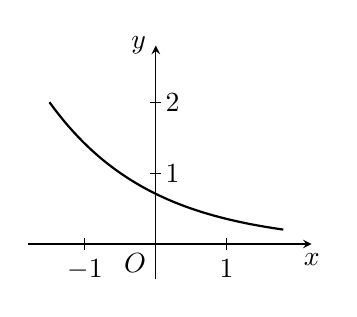
\begin{tikzpicture}[>=stealth, scale=0.9]
  % 坐标轴
  \draw[->] (-1.8, 0) -- (2.2, 0) node[below] {$x$};
  \draw[->] (0, -0.5) -- (0, 2.8) node[left] {$y$};
  \node[below left] at (0, 0) {$O$};

  % 刻度
  \draw (-1, 0.08) -- (-1, -0.08) node[below] {$-1$};
  \draw (1, 0.08) -- (1, -0.08) node[below] {$1$};
  \draw (0.08, 1) -- (-0.08, 1);
  \node[right] at (0, 1) {$1$};
  \draw (0.08, 2) -- (-0.08, 2);
  \node[right] at (0, 2) {$2$};

  % 指数函数曲线 (a=0.5, b=-0.5 即 y = 0.5^(x + 0.5))
  \draw[thick, domain=-1.5:1.8, samples=50] plot (\x, {pow(0.5, \x + 0.5)});
\end{tikzpicture}
\end{center}
\nopagebreak[4]
\begin{gkopts}(2)
\task A．$a > 1, b < 0$
\task B．$a > 1, b > 0$
\task C．$0 < a < 1, b > 0$
\task D．$0 < a < 1, b < 0$
\end{gkopts}

\Needspace{0.4\textheight}
\end{question}
\begin{question}
\gkti{6}若函数 $y = \sin(\omega x + \varphi) \; (x \in \mathbf{R}, \omega > 0, 0 \leqslant \varphi < 2\pi)$ 的部分图象如图，则\mbox{（　　）}
\nopagebreak[4]
\begin{center}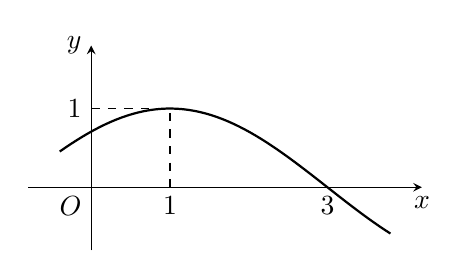
\begin{tikzpicture}[>=stealth, scale=1.0]
  % 坐标轴
  \draw[->] (-0.8, 0) -- (4.2, 0) node[below] {$x$};
  \draw[->] (0, -0.8) -- (0, 1.8) node[left] {$y$};
  \node[below left] at (0, 0) {$O$};

  % 刻度与虚线
  \node[left] at (0, 1) {$1$};
  \node[below] at (1, 0) {$1$};
  \node[below] at (3, 0) {$3$};

  \draw[dashed] (0, 1) -- (1, 1) -- (1, 0);

  % 正弦函数曲线: y = sin(pi/4 * x + pi/4)
  \draw[thick, domain=-0.4:3.8, samples=60] plot (\x, {sin((\x * 0.25 + 0.25) * 180)});
\end{tikzpicture}
\end{center}
\nopagebreak[4]
\begin{gkopts}(1)
\task A．$\omega = \dfrac{\pi}{2}, \varphi = \dfrac{\pi}{4}$
\task B．$\omega = \dfrac{\pi}{3}, \varphi = \dfrac{\pi}{6}$
\task C．$\omega = \dfrac{\pi}{4}, \varphi = \dfrac{\pi}{4}$
\task D．$\omega = \dfrac{\pi}{4}, \varphi = \dfrac{5\pi}{4}$
\end{gkopts}

\end{question}
\begin{question}
\gkti{7}已知 $p: |2x - 3| < 1$，$q: x(x - 3) < 0$，则 $p$ 是 $q$ 的\mbox{（　　）}

\begin{gkopts}(2)
\task A．充分不必要条件
\task B．必要不充分条件
\task C．充要条件
\task D．既不充分也不必要条件
\end{gkopts}

\Needspace{0.4\textheight}
\end{question}
\begin{question}
\gkti{8}如图，长方体 $ABCD - A_1B_1C_1D_1$ 中，$AA_1 = AB = 2$，$AD = 1$，点 $E$、$F$、$G$ 分别是 $DD_1$、$AB$、$CC_1$ 的中点，则异面直线 $A_1E$ 与 $GF$ 所成的角是\mbox{（　　）}
\nopagebreak[4]
\begin{center}\begin{tikzpicture}[>=stealth, scale=1.0]
  % 顶点定义
  \coordinate (A) at (0, 0);
  \coordinate (B) at (2.4, 0);
  \coordinate (C) at (3.4, 0.8);
  \coordinate (D) at (1.0, 0.8);
  \coordinate (A1) at (0, 2.2);
  \coordinate (B1) at (2.4, 2.2);
  \coordinate (C1) at (3.4, 3.0);
  \coordinate (D1) at (1.0, 3.0);

  % 中点定义
  \coordinate (E) at ($(D)!0.5!(D1)$);
  \coordinate (F) at ($(A)!0.5!(B)$);
  \coordinate (G) at ($(C)!0.5!(C1)$);

  % 可见实线
  \draw[thick] (A) -- (B) -- (C) -- (C1) -- (D1) -- (A1) -- cycle;
  \draw[thick] (B) -- (B1) -- (C1);
  \draw[thick] (A1) -- (B1);

  % 不可见虚线
  \draw[thick, dashed] (A) -- (D) -- (C);
  \draw[thick, dashed] (D) -- (D1);

  % 异面直线连接
  \draw[thick, dashed] (A1) -- (E);
  \draw[thick, dashed] (G) -- (F);

  % 顶点标签
  \node[below left] at (A) {$A$};
  \node[below right] at (B) {$B$};
  \node[right] at (C) {$C$};
  \node[above left] at (D) {$D$};
  \node[above left] at (A1) {$A_1$};
  \node[below left] at (B1) {$B_1$};
  \node[above right] at (C1) {$C_1$};
  \node[above left] at (D1) {$D_1$};
  \node[right] at (E) {$E$};
  \node[below] at (F) {$F$};
  \node[right] at (G) {$G$};
\end{tikzpicture}
\end{center}
\nopagebreak[4]
\begin{gkopts}(2)
\task A．$\arccos\dfrac{\sqrt{15}}{5}$
\task B．$\dfrac{\pi}{4}$
\task C．$\arccos\dfrac{\sqrt{10}}{5}$
\task D．$\dfrac{\pi}{2}$
\end{gkopts}

\end{question}
\begin{question}
\gkti{9}从 6 人中选 4 人分别到巴黎、伦敦、悉尼、莫斯科四个城市游览，要求每个城市有一人游览，每人只游览一个城市，且这 6 人中甲、乙两人不去巴黎游览，则不同的选择方案共有\mbox{（　　）}

\begin{gkopts}(4)
\task A．$300$ 种
\task B．$240$ 种
\task C．$144$ 种
\task D．$96$ 种
\end{gkopts}

\end{question}
\begin{question}
\gkti{10}已知 $F_1$、$F_2$ 是双曲线 $\dfrac{x^2}{a^2} - \dfrac{y^2}{b^2} = 1 \; (a > 0, b > 0)$ 的两焦点，以线段 $F_1F_2$ 为边作正三角形 $MF_1F_2$，若边 $MF_1$ 的中点在双曲线上，则双曲线的离心率是\mbox{（　　）}

\begin{gkopts}(2)
\task A．$4 + 2\sqrt{3}$
\task B．$\sqrt{3} - 1$
\task C．$\dfrac{\sqrt{3} + 1}{2}$
\task D．$\sqrt{3} + 1$
\end{gkopts}

\end{question}
\begin{question}
\gkti{11}设 $a, b \in \mathbf{R}$，$a^2 + 2b^2 = 6$，则 $a + b$ 的最小值是\mbox{（　　）}

\begin{gkopts}(2)
\task A．$-2\sqrt{2}$
\task B．$-\dfrac{5\sqrt{3}}{3}$
\task C．$-3$
\task D．$-\dfrac{7}{2}$
\end{gkopts}

\end{question}
\begin{question}
\gkti{12}$f(x)$ 是定义在 $\mathbf{R}$ 上的以 3 为周期的奇函数，且 $f(2) = 0$，则方程 $f(x) = 0$ 在区间 $(0, 6)$ 内解的个数的最小值是\mbox{（　　）}

\begin{gkopts}(4)
\task A．$2$
\task B．$3$
\task C．$5$
\task D．$7$
\end{gkopts}

\end{question}
\gkpart{二、填空题（本大题共 4 小题，每小题 4 分，共 16 分）}

\begin{question}
\gkti{13}$\left(2\sqrt{x} - \dfrac{1}{x}\right)^6$ 展开式中的常数项是 $\underline{\qquad\qquad}$．（用数字作答）

\end{question}
\begin{question}
\gkti{14}非负实数 $x, y$ 满足 $\begin{cases} 2x + y \leqslant 0, \\ x + y - 3 \leqslant 0, \end{cases}$ 则 $x + 3y$ 的最大值为 $\underline{\qquad\qquad}$．

\end{question}
\begin{question}
\gkti{15}若常数 $b$ 满足 $|b| > 1$，则 $\lim\limits_{n\to\infty} \dfrac{1 + b + b^2 + \dots + b^{n-1}}{b^n} = \underline{\qquad\qquad}$．

\end{question}
\begin{question}
\gkti{16}把下面不完整的命题补充完整，并使之成为真命题：
若函数 $f(x) = 3 + \log_2 x$ 的图象与 $g(x)$ 的图象关于 $\underline{\qquad\qquad}$ 对称，则函数 $g(x) = \underline{\qquad\qquad}$．
注：填上你认为可以成为真命题的一件情形即可，不必考虑所有可能的情形．

\end{question}
\gkpart{三、解答题（本大题共 6 小题，共 74 分）}

\begin{question}
\gkti{17}已知 $-\dfrac{\pi}{2} < x < 0$，$\sin x + \cos x = \dfrac{1}{5}$．
(1) 求 $\sin x - \cos x$ 的值；
\Needspace{5\baselineskip}
(2) 求
\nopagebreak[4]
\[
\frac{3\sin^2\dfrac{x}{2} - 2\sin\dfrac{x}{2}\cos\dfrac{x}{2} + \cos^2\dfrac{x}{2}}{\tan x + \cot x}
\]
的值．

\end{question}
\begin{question}
\gkti{18}甲、乙两人在罚球线投球命中的概率分别为 $\dfrac{1}{2}$ 与 $\dfrac{2}{5}$，投中得 1 分，投不中得 0 分．
(1) 甲、乙两人在罚球线各投球一次，求两人得分之和 $\xi$ 的数学期望；
(2) 甲、乙两人在罚球线各投球二次，求这四次投球中至少一次命中的概率．

\end{question}
\begin{question}
\gkti{19}已知函数 $f(x) = \dfrac{ax - 6}{x^2 + b}$ 的图象在点 $M(-1, f(-1))$ 处的切线方程为 $x + 2y + 5 = 0$．
(1) 求函数 $y = f(x)$ 的解析式；
(2) 求函数 $y = f(x)$ 的单调区间．

\Needspace{0.4\textheight}
\end{question}
\begin{question}
\gkti{20}如图，直二面角 $D - AB - E$ 中，四边形 $ABCD$ 是边长为 2 的正方形，$AE = EB$，$F$ 为 $CE$ 上的点，且 $BF \perp \text{\text{平面} } ACE$．
\nopagebreak[4]
\begin{center}\begin{tikzpicture}[>=stealth, scale=1.0]
  % 顶点定义
  \coordinate (A) at (0, 0);
  \coordinate (B) at (2.8, 0);
  \coordinate (C) at (2.8, 2.8);
  \coordinate (D) at (0, 2.8);
  \coordinate (E) at (1.0, -0.7);
  \coordinate (F) at ($(C)!0.68!(E)$);

  % 可见实线
  \draw[thick] (D) -- (C) -- (B) -- (E) -- (A) -- (D);
  \draw[thick] (D) -- (E);
  \draw[thick] (C) -- (E);
  \draw[thick] (B) -- (F);

  % 不可见虚线
  \draw[thick, dashed] (A) -- (B);
  \draw[thick, dashed] (A) -- (C);

  % 顶点标签
  \node[above left] at (D) {$D$};
  \node[above right] at (C) {$C$};
  \node[below left] at (A) {$A$};
  \node[below right] at (B) {$B$};
  \node[below] at (E) {$E$};
  \node[left] at (F) {$F$};
\end{tikzpicture}
\end{center}
\nopagebreak[4]
(1) 求证 $AE \perp \text{\text{平面} } BCE$；
(2) 求二面角 $B - AC - E$ 的大小；
(3) 求点 $D$ 到平面 $ACE$ 的距离．

\end{question}
\begin{question}
\gkti{21}已知方向向量为 $\vec{v} = (1, \sqrt{3})$ 的直线 $l$ 过点 $(0, -2\sqrt{3})$ 和椭圆 $C: \dfrac{x^2}{a^2} + \dfrac{y^2}{b^2} = 1 \; (a > b > 0)$ 的焦点，且椭圆 $C$ 的中心关于直线 $l$ 的对称点在椭圆 $C$ 的右准线上．
(1) 求椭圆 $C$ 的方程；
(2) 是否存在过点 $E(-2, 0)$ 的直线 $m$ 交椭圆 $C$ 于点 $M$、$N$，满足 $\overrightarrow{OM} \cdot \overrightarrow{ON} = \dfrac{4}{3}\sqrt{6}\cot\angle MON \neq 0$（$O$ 为原点）．若存在，求直线 $m$ 的方程；若不存在，请说明理由．

\end{question}
\begin{question}
\gkti{22}已知数列 $\{a_n\}$ 满足 $a_1 = a$，$a_{n+1} = 1 + \dfrac{1}{a_n}$．我们知道当 $a$ 取不同的值时，得到不同的数列，如当 $a = 1$ 时，得到无穷数列：$1, 2, \dfrac{3}{2}, \dfrac{5}{3}, \dots$；当 $a = -\dfrac{1}{2}$ 时，得到有穷数列：$-\dfrac{1}{2}, -1, 0$．
(1) 求当 $a$ 为何值时 $a_4 = 0$；
(2) 设数列 $\{b_n\}$ 满足 $b_1 = -1$，$b_{n+1} = \dfrac{1}{b_n - 1} \; (n \in \mathbf{N}_+)$，求证 $a$ 取数列 $\{b_n\}$ 中的任一个数，都可以得到一个有穷数列 $\{a_n\}$；
(3) 若 $\dfrac{3}{2} < a_n < 2 \; (n \geqslant 4)$，求 $a$ 的取值范围．

\end{question}